\chapter{An\'alisis temporal y costes de desarrollo}\label{anatemporal}
\section{An\'alisis temporal}
\subsection{Iteraciones}

Dividiremos el trabajo en varias iteraciones, de forma que el proyecto se quede lo más planificado posible para que, a la hora de trabajar, solo haya que seguir las iteraciones:\\

\textbf{Iteración 1}\\

En esta iteración buscamos dejar empezado tanto el proyecto como la documentación, creando una base sobre la que trabajar más adelante. Además dejamos preparadas las herramientas a utilizar, tanto de trabajo (Eclipse IDE, Microsoft Visual Studio Code), como de redacción (TeXStudio, Google Docs), almacenamiento en la nube (GitHub, Google Drive) y gestión del tiempo (Toggl). Realizamos el primer capítulo de la documentación y diseñamos los mockups.\\

\textbf{Iteración 2}\\

Planificamos el proyecto de forma que se quede dividido para las siguientes iteraciones y continuamos con la documentación. Redactamos los apartados que podemos (ya que algunos de ellos requieren que se haya avanzado más) de los capítulos 2, 3, 4 y 5. Además se realiza un curso de Angular para prepararnos para la siguiente iteración.\\

\textbf{Iteración 3 --TODO}\\

Página de inicio, registro de usuario, acceso a perfil y base de datos, se realiza la vista de la página de inicio y los elementos back-end necesarios para gestionar usuarios y permitirles registrarse y acceder a su perfil. Se realizan las pruebas respectivas.\\

\textbf{Iteración 4 --TODO}\\

Implementar api y los elementos relacionados con esta, se implementan los elementos necesarios para disponer de la información que nos provee la api y se crean todas las funcionalidades que la requieren. Se realizan las pruebas respectivas.\\

\textbf{Iteración 5 --TODO}\\

Implementar JSON’s y vistas relacionadas con estos, se añaden los JSON’s que poseemos con información no disponible en la api y se realizan las funcionalidades que esta nueva información nos permite. Se realizan las pruebas respectivas.\\

\textbf{Iteración 6 --TODO}\\

Vestuario, se realiza la funcionalidad del vestuario. Se realizan las pruebas respectivas.\\

\textbf{Iteración 7 --TODO}\\

Nabos, diseños y código de sueño, se realizan las funcionalidades para calcular precios de nabos y compartir diseños y códigos de sueño. Se realizan las pruebas respectivas.\\

\textbf{Iteración 8 --TODO}\\

Terminar la documentación, realizar los apartados restantes de la documentación para dar por cerrado el proyecto.\\

\subsection{Estimación vs Realidad}

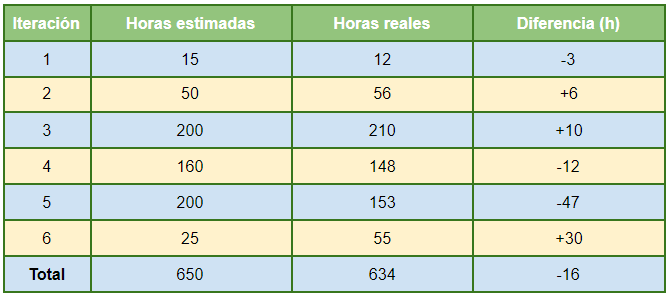
\includegraphics[width=\textwidth]{img/cap4/analisistiempo.jpg}

\section{Costes de desarrollo}
	
\subsection{Costes Directos}	

\textbf{Personal}

Dado que aunque sepamos algo de Spring gracias a las asignaturas cursadas anteriormente (Diseño y pruebas I y II), no tenemos ninguna experiencia con Angular, calcularemos nuestros sueldos clasificándonos como programadores junior. Dicho conjunto cobra una media de 19.000€ al año, lo cual sería 1.584€ al mes, que al dividirlos en un horario de trabajo de 40 horas semanales, 160 horas al mes, equivaldría a 10€ la hora.\\

Esto hay que multiplicarlo por dos ya que el equipo del proyecto está formado por dos personas, es decir, dos programadores junior con sus respectivos sueldos, por lo que sería un total de 20€ la hora.\\

\subsection{Costes Indirectos}

Realizaremos el proyecto en Eclipse y en Microsoft Visual Studio Code, ambos entornos de desarrollo gratuitos, en una base de Spring con Angular y con una base de datos de TODOOOOOOOO, cuyas licencias son gratuitas.\\

Para el almacenamiento de datos en la nube usaremos GitHub y Google Drive, los cuales disponen de licencia gratuita con aspectos limitados.\\

Para la redacción utilizaremos tanto Google Docs como TeXStudio, ambos con licencia gratuita.\\

Para la gestión de tiempo y comunicación usaremos Toggl y WhatsApp respectivamente, las cuales también disponen de licencia gratuita (con limitaciones en el caso de Toggl).\\

Los únicos costes indirectos que podríamos encontrar sería la electricidad y la conexión a Internet, lo cual supone de media 35€ por persona, 70€ en total al mes.\\

\subsection{Amortizaciones}

Para realizar el proyecto hemos usado los siguientes equipos:\\

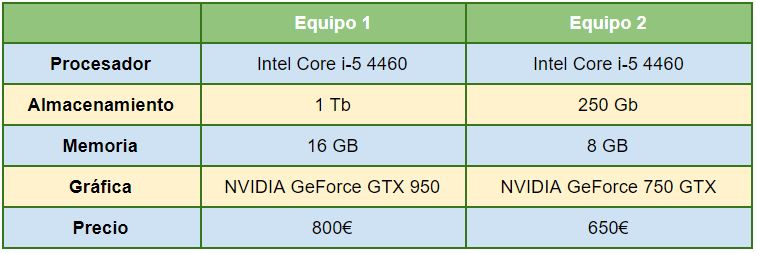
\includegraphics[width=\textwidth]{img/cap4/equipos.jpg}

\bigskip

Además de esto para comunicarnos hemos usado nuestros teléfonos móviles, por eso hemos decidido añadirlo al documento:\\

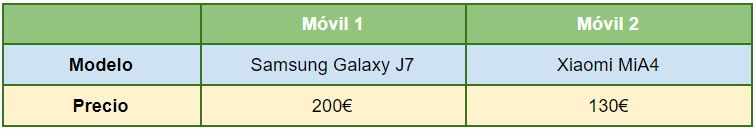
\includegraphics[width=\textwidth]{img/cap4/moviles.jpg}


\subsection{Total}	

Finalmente, sumaremos todos los cálculos anteriores para dar una cifra al precio total:\\

TODO TABLA TOTAL



	

	